\documentclass[11pt]{article}
\usepackage{tikz}
\usepackage{tkz-euclide}
\usetikzlibrary{arrows}
\begin{document}

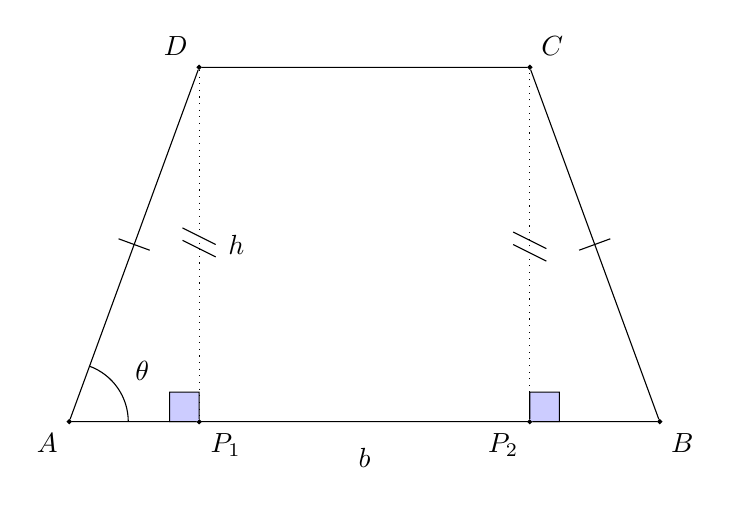
\begin{tikzpicture}[scale=1.5,>=stealth,point/.style={draw,circle,fill = black,inner sep=0.5pt},]
      
%Labeling points
\node (A) at (0, 0)[point,label=below left:$A$] {};
\node (B) at (5, 0)[point,label=below right:$B$] {};
\node (C) at (3.9, 3)[point,label=above right:$C$] {};
\node (D) at (1.1, 3)[point,label=above left:$D$] {};
\node (P1) at (1.1, 0)[point,label=below right:$P_1$] {};
\node (P2) at (3.9, 0)[point,label=below left:$P_2$] {};

%Drawing quad ABCD
\draw (A) -- node[below=6pt]{$b$}(B) -- (C) -- (D) -- (A);
\draw[dotted] (D) -- node[right = 7pt]{$h$}(P1)(P2)--(C);

%marking line segment
\tkzMarkSegments[mark=|,size=6pt](A,D C,B)
\tkzMarkSegments[mark=s||,size=6pt](P1,D C,P2)

%marking angles
\tkzMarkAngle[fill=orange!40,size=0.5cm,mark=](P1,A,D)
\tkzMarkRightAngle[fill=blue!20](D,P1,A)
\tkzMarkRightAngle[fill=blue!20](C,P2,B)
\tkzLabelAngle[pos=0.75](P1,A,D){$\theta$}

\end{tikzpicture} 

\end{document}

